%%%%%%%%%%%%%%%%%%%%%%%%%%% asme2e.tex %%%%%%%%%%%%%%%%%%%%%%%%%%%%%%%
% Template for producing ASME-format articles using LaTeX            %
% Written by   Harry H. Cheng                                        %
%              Integration Engineering Laboratory                    %
%              Department of Mechanical and Aeronautical Engineering %
%              University of California                              %
%              Davis, CA 95616                                       %
%              Tel: (530) 752-5020 (office)                          %
%                   (530) 752-1028 (lab)                             %
%              Fax: (530) 752-4158                                   %
%              Email: hhcheng@ucdavis.edu                            %
%              WWW:   http://iel.ucdavis.edu/people/cheng.html       %
%              May 7, 1994                                           %
% Modified: February 16, 2001 by Harry H. Cheng                      %
% Modified: January  01, 2003 by Geoffrey R. Shiflett                %
% Use at your own risk, send complaints to /dev/null                 %
%%%%%%%%%%%%%%%%%%%%%%%%%%%%%%%%%%%%%%%%%%%%%%%%%%%%%%%%%%%%%%%%%%%%%%

%%% use twocolumn and 10pt options with the asme2e format
\documentclass[twocolumn,10pt]{asme2e}
\special{papersize=8.5in,11in}
\usepackage{fancyvrb}
\usepackage{graphicx}
\usepackage{amsmath}
\usepackage{tikz}
\usepackage{pgf}
\usepackage{cite}
\usetikzlibrary{arrows}
\usetikzlibrary{snakes}
\renewcommand{\b}[1]{\mathbf{#1}}
\newcommand{\bs}[1]{\boldsymbol{#1} }
\newcommand{\uv}[1]{\hat{\mathbf{#1}}}
\newcommand{\drawpendulum}[6]{
  \def \x {#1}
  \def \y {#2}
  \def \theta {#3}
  \def \length {#4}
  \def \m {#5}
  \def \index {#6}
  % Shift the origin to x, y
  \pgftransformshift{\pgfpoint{\x}{\y}}
  % Draw a dashed line from origin to -l
  \draw[dashed] (0,0)--(0,-\length);
  % Draw an arc from (0,-.75*l) that is theta degrees clockwise
  \draw[->] (0,-0.75*\length) arc (-90:\theta-90:0.75*\length);
  % Rotate to middle of arc and label it
  \pgftransformrotate{\theta/2}
  \node at (0,-0.90*\length) {$q_{\scriptscriptstyle\index}$};
  % Rotate to end of arc
  \pgftransformrotate{\theta/2}
  % Draw the link
  \draw [thick] (0,0)--(0,-\length);
  % Label the link
  \draw[snake=brace] (\m+1mm,0)--(\m+1mm,-\length);
  \node at (\m+6mm,-0.5*\length) {$l_{\scriptscriptstyle\index}$};
  % Draw the mass
  \shade[ball color=black] (0,-\length) circle (\m);
  % Label the mass
  \pgftransformshift{\pgfpoint{0}{-\length}}
  \pgftransformrotate{-\theta}
  \node at (-\m/2-2mm, -\m/2-2mm) {$m_{\scriptscriptstyle\index}$};
  \pgftransformrotate{\theta}
  \pgftransformshift{\pgfpoint{0}{\length}}

  % Reset the coordinates back to what they were prior to this command
  \pgftransformrotate{-\theta}
  \pgftransformshift{\pgfpoint{-\x}{-\y}}
}

%% The class has several options
%  onecolumn/twocolumn - format for one or two columns per page
%  10pt/11pt/12pt - use 10, 11, or 12 point font
%  oneside/twoside - format for oneside/twosided printing
%  final/draft - format for final/draft copy
%  cleanfoot - take out copyright info in footer leave page number
%  cleanhead - take out the conference banner on the title page
%  titlepage/notitlepage - put in titlepage or leave out titlepage
%
%% The default is oneside, onecolumn, 10pt, final

%%% Replace here with information related to your conference
\confshortname{IDETC/CIE 2013}
\conffullname{the ASME 2013 International Design Engineering Technical Conferences \&\\
              Computers and Information in Engineering Conference}

%%%%% for date in a single month, use
%\confdate{24-28}
%\confmonth{September}
%%%%% for date across two months, use
\confdate{4-7}
\confdate{August}
\confyear{2013}
\confcity{Portland}
\confcountry{USA}

%%% Replace DETC2009/MESA-12345 with the number supplied to you
%%% by ASME for your paper.
\papernum{IDETC/CIE 2013-13470}

%%% You need to remove 'DRAFT: ' in the title for the final submitted version.
\title{DRAFT: Constrained Multibody Dynamics With Python: From Symbolic
Equation Generation to Publication}

%%% first author
\author{Gilbert Gede\thanks{Address all correspondence to this author}, Dale L.
Peterson, Angadh S. Nanjangud, Jason K. Moore, Mont Hubbard
  \affiliation{
    Sports Biomechanics Laboratory\\
    Department of Mechanical and Aerospace Engineering\\
    University of California\\
    Davis, California 95616\\
    Email: \{ggede, dlpeterson, asnanjangud, jkmoor, mhubbard\}@ucdavis.edu
  }
}

\begin{document}

\maketitle

%%%%%%%%%%%%%%%%%%%%%%%%%%%%%%%%%%%%%%%%%%%%%%%%%%%%%%%%%%%%%%%%%%%%%%
\begin{abstract}
% Context
\it Symbolic equations of motion (EOMs) for multibody systems are desirable
for simulation, stability analyses, control system design, and parameter
studies.
% Need  (what we have and what we want)
Despite this, the majority of engineering software designed to analyze
multibody systems are numeric in nature (or present a purely numeric user
interface). To our knowledge, none of the existing software packages are 1)
fully symbolic, 2) open source, and 3) implemented in a popular, general,
purpose high level programming language.
% Task
In response, we extended SymPy (an existing computer algebra system implemented
in Python) with functionality for derivation of symbolic EOMs for constrained
multibody systems with many degrees of freedom.
% Object of the document
We present the design and implementation of the software and cover the basic
usage and workflow for solving and analyzing problems. The intended audience is
the academic research community, graduate and advanced undergraduate students,
and those in industry analyzing multibody systems.
% Findings
We demonstrate the software by deriving the EOMs of a N-link pendulum, show its
capabilities for \LaTeX output, and how it integrates with other Python
scientific libraries - allowing for numerical simulation, publication quality
plotting, animation, and online notebooks designed for sharing results.
% Conclusion
This software fills a unique role in dynamics and is attractive to academics
and industry because of its BSD open source license which permits open source
or commercial use of the code.
% TODO cite BSD license

% Perspectives
\end{abstract}

%%%%%%%%%%%%%%%%%%%%%%%%%%%%%%%%%%%%%%%%%%%%%%%%%%%%%%%%%%%%%%%%%%%%%%
\section*{INTRODUCTION}
There are many dynamic systems which can be better or more effectively studied
when their EOMs are accessible in a symbolic form. For equations that may be
visually inspected (i.e., of reasonable length), symbolics are generally
preferable because the interrelations of the variables and constants can give
clear understanding to the nature of the problem without the need for numerical
simulation. Many classic problems fit this category, such as the
mass-spring-damper, double pendulum, rolling disc, rattleback, and tippy-top.
The benefits of symbolic equations of motion are not limited to these basic
problems though. Larger, more complicated multibody systems can also be studied
more effectively when the equations of motion are available symbolically.
Advanced simplification routines can sometimes reduce the length of the
equations to a human readable size. Even if the final equations of motion are
too lengthy for human consumption, the symbolic nature of the steps to get to
the equations of motion are short enough that symbolic checks can be used to
validate the correctness of the derivation. Problems in biomechanics,
spacecraft dynamics, and single-track vehicles have all been sucessfully
studied using symbolic EOMs.

Having the symbolic equations of motion available permits numerical simulation,
but also allows for a more mathematical study of the system in question. System
behavior can be studied parametrically by examining coefficients in the
differential equations. This includes symbolic expressions for equilibria
points and symbolic conditions for the stability of these points. The symbolic
form also allows for more complicated tasks, such as analyzing how
infinitesimal changes in system parameters (masses, lengths, inertias) affect
the dynamics, studying lumped parameter discretization sizing, and analyzing
how coordinate choices affect problem complexity or configuration
singularities. It also becomes possible to share the equations of motion in a
``written'' form to other individuals for collaboration, validation, or
comparison reasons. This allows for the EOMs to be used with other software
packages, for multi-domain simulation, hardware-in-the-loop testing, or for use
in optimal control/optimization problems.

Before adequate computing technology was available, the equations of motion for
multibody dynamics problems were formed by hand. There are many methodologies
to obtain the correct equations of motion (Newton-Euler, Lagrange, Kane,
Hamilton, etc). But all methods are tedious and error-prone when derived by
hand, which limits the size and complexity of systems which can be studied. It
only takes a handful of unique orientations between a small set of rigid bodies
within the system to reach this point of complexity. The introduction of
computer algebra systems (CAS) has reduced the difficulty involved in forming
the equations of motion, but it has not completely eliminated these problems.
However, the details of the symbolic algebra, differentiation, and vector
calculus can be handled by a reliable CAS, eliminating the errors associated
with those operations - allowing the user to think more about the implications
of the dynamic equations.

The software presented herein addresses some of the limitations of hand
derivations and allows for the symbolic study of complex multibody dynamics
problems. There already exist software packages which similarly meet these
limited criteria (e.g. Autolev/MotionGenesis, AutoSim/VehicleSim). But when
developing our software, we also included these unique requirements:
\begin{enumerate}
  \item The software should be open source with a liberal license, encourage
  collaborative development, ensure continued project development is not
  limited by or relying on any individual or organization, and allow easy
  integration and use by other projects.

  \item The software should be written in a popular high level programming
  language that balances efficient execution speed with efficient programmer
  development time, and has a wide selection of scientific libraries (or can
  conveniently interface with libraries written in other languages).

  \item The software should be built on top of an existing full-featured
  symbolic CAS that is also open source.

  \item The software should easily export the equations in formats that are
  publication friendly (i.e., \LaTeX) or are compatible with other populer
  computing platforms and languages (i.e., modelica, C/C++/Fortan, MATLAB).
\end{enumerate}

To meet these criteria, we selected Python as the programming language to
implement our software. Python is interactive, high level, easy to learn,
widely available, widely used (it is one of the top four languages supported at
Google), cross platform, open source, and has a large scientific user base.
% TODO cite google factoid.

Our software is distributed as a sub-package of SymPy \cite{sympy2012}, which
is a full featured CAS written in Python. SymPy is part of the SciPy Stack
\cite{SciPyStackGithub} specification and is included with all scientific
Python distributions including Enthought, Sage, Anaconda, and Python(x,y).
SymPy is one of the more actively developed Python packages with a large number
of maintainers, ensuring a long future. The SymPy development model allows new
functionality to be easily added and allows for other users to view our code,
suggest additional abilities, and improve upon and add to what we have already
done, as well as ensure that the our code is constantly tested against any
changes or updates to the base symbolic functionality offered by SymPy.

In this paper, we discuss two main topics: 1) The interface to the EoM
generation sub-package sympy.physics.mechanics, and 2) the workflow for
studying multibody dynamic systems (from derivation to simulation and
visualization), which we call Python Dynamics (PyDy). We will explore these two
topics through an explanation of the software design and by demonstrating a
test problem which displays software functionality and usage, how our software
is incorporated into a workflow for analyzing dynamic systems, and the results
of these processes. We will then discuss a number of other features, internal
constructions within our software, and verification with benchmark examples.

%%%%%%%%%%%%%%%%%%%%%%%%%%%%%%%%%%%%%%%%%%%%%%%%%%%%%%%%%%%%%%%%%%%%%%
\section*{DEMONSTRATION PROBLEM}
We now demonstrate the value of PyDy through the derivation of the $N$-pendulum
system shown in Figure (\ref{fig:n_pendulum}).  The system is defined by $N$
massless links of length $l_i$ with particles of mass $m_i$ fixed at one end.
We selected this problem because it illustrates the power and utility of having
EoM generation code available within a full-featured programming language. The
angular velocity of each and every link must be found, as well as the velocity
of each particle. The velocity of $i$-th particle is
\begin{align*}
  %\omega_i &= u_i \cdot a_z\\
  \underline{v}_i &= \underline{v}_{i-1} + \underline{\omega}_i \times
  \underline{r}^i \qquad (i = 1,\dots,N)
\end{align*}

This nesting of velocities is best addressed with a loop, something
that a computer is well suited for (loop unrolling is difficult by hand when
there are many steps and $N$ is large). The 37 lines of source code required to
derive the dynamic equations of motion for the $N$ pendulum, where $N$ is
the number of links, is shown in figure \ref{fig:n_pendulum_source}.

The script first imports necessary functions and classes, then declares a
number of symbolic variables that represent generalized coordinates,
generalized speeds, constant parameters, reference frames, points and
particles. A few empty lists are created before the for loop is entered; these
lists are filled by the loop.  When the final iteration of the for loop is
complete, the kinematics and all active forces of the problem have been
completely specified. The last two lines of the script take this specification
of kinematics and dynamics and generate Kane's dynamical equations of motion
($F_r + F_r^* = 0$) in symbolic form. At this point, these equations may be
manipulated as fully symbolic variables for a variety of purposes. For example,
the command \verb|mlatex(fr)| generates \LaTeX code for the generalized active
force $F_r$, which renders as:
\begin{equation}
\left[\begin{smallmatrix}g l_{0} m_{0} \operatorname{sin}\left(q_{0}\right) + g l_{0} m_{1} \operatorname{sin}\left(q_{0}\right) + g l_{0} m_{2} \operatorname{sin}\left(q_{0}\right) + g l_{0} m_{3} \operatorname{sin}\left(q_{0}\right)\\g l_{1} m_{1} \operatorname{sin}\left(q_{1}\right) + g l_{1} m_{2} \operatorname{sin}\left(q_{1}\right) + g l_{1} m_{3} \operatorname{sin}\left(q_{1}\right)\\g l_{2} m_{2} \operatorname{sin}\left(q_{2}\right) + g l_{2} m_{3} \operatorname{sin}\left(q_{2}\right)\\g l_{3} m_{3} \operatorname{sin}\left(q_{3}\right)\end{smallmatrix}\right]
\end{equation}
with no further modification from the user.

\begin{figure}
\begin{center}
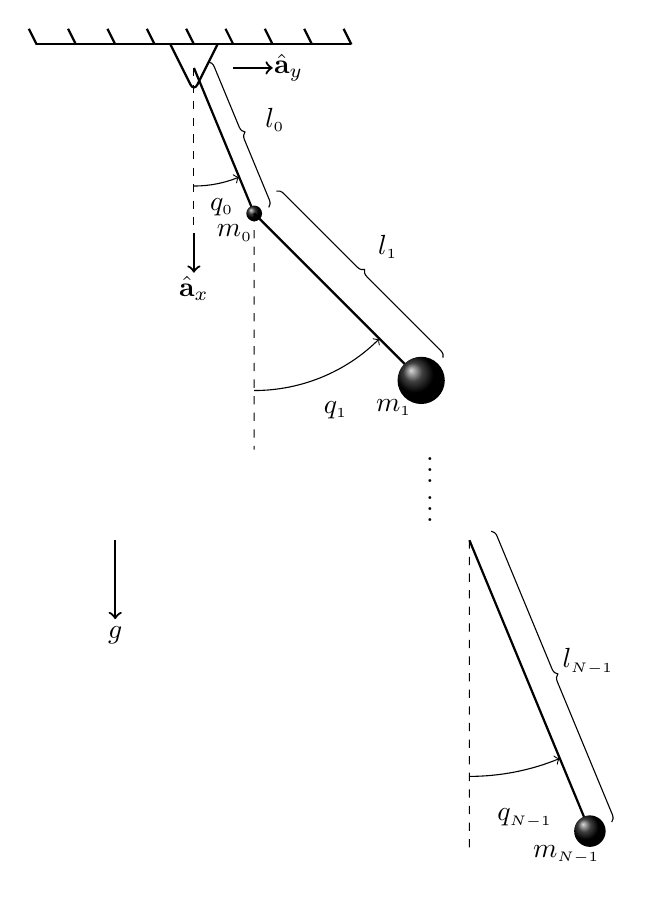
\begin{tikzpicture}[scale=1.0]
    \draw [thick] (-2cm,3mm)--(2cm,3mm);
    \draw [thick, rounded corners=1mm] (-3mm,3mm)--(0,-3mm)--(3mm,3mm);
    \draw [->,thick] (5mm,0)--(10mm,0);
    \node at (12mm,0) {$\hat{\mathbf{a}}_y$};
    \draw [->,thick] (0,-21mm)--(0,-26mm);
    \node at (0,-28mm) {$\hat{\mathbf{a}}_x$};
    \draw [->,thick] (-10mm,-60mm)--(-10mm,-70mm);
    \node at (-10mm,-72mm) {$g$};
   %\drawpendulum{  x}{  y}{ deg}{  l}{  m}{i}
    \drawpendulum{0cm}{0cm}{22.5}{2cm}{1mm}{0}
    \drawpendulum{0.76536686cm}{-1.847759cm}{45}{3cm}{3mm}{1}
    \node at (3cm,-5cm) {$\vdots$};
    \node at (3cm,-5.5cm) {$\vdots$};
    \drawpendulum{3.5cm}{-6cm}{22.5}{4cm}{2mm}{N-1}
    \foreach \x in {-2cm,-1.5cm,-1.0cm,-0.5cm,0cm,0.5cm,1.0cm,1.5cm,2cm}
      \draw[thick] (\x,3mm)--(\x-1mm,5mm);
\end{tikzpicture}
\end{center}
\caption{N-pendulum system, a sequence of massive links connected by revolute
joints subjected to a gravitational field.}
\label{fig:n_pendulum}
\end{figure}

\begin{figure*}
\fvset{frame=single}
\VerbatimInput{n_pends_minimal.py}
\caption{User Python script to derive equations of motion for N-pendulum}
\label{fig:n_pendulum_source}
\end{figure*}

There are other options besides \LaTeX output which are useful. Within a
console, commands to ``pretty print'' symbolic expressions can be performed
with \verb|mpprint|, which generates the output formatted just like the
\LaTeX equation above, but within the terminal.

Another part of studying dynamic systems is simulation and visualization of the
results. SymPy can only analytically solve simple ODEs, so the equations of
motion generated for more complex systems need to be passed to other numerical
integrators. Currently, sympy.physics.mechanics can make use of existing SymPy
translation functions, but more advanced options to generate compiled code are
being developed and guided by user demands. The SymPy translation function
\verb|lambdify| can convert symbolic expressions to a function using NumPy
code. The code in figure \ref{fig:numerical_code} (which is executed after the
previously written code) shows this.

\begin{figure*}
\begin{Verbatim}[frame=single]
from pylab import *
from sympy import Dummy, lambdify
from scipy.integrate import odeint

parameters = [g]                                             # Parameter Definitions
parameter_vals = [9.81]                                      # First we define gravity
for i in range(N):
    parameters += [l[i], m[i]]                               # Then each mass
    parameter_vals += [1. / N, 0.01 / N]                     # and length

dummy_symbols = [Dummy() for i in q + u]                     # Necessary to translate
dummy_dict = dict(zip(q + u, dummy_symbols))                 # out of functions of time
kds = KM.kindiffdict()                                       # Need to eliminate qdots
MM = KM.mass_matrix_full.subs(kds).subs(dummy_dict)          # Substituting away qdots
Fo = KM.forcing_full.subs(kds).subs(dummy_dict)              # and in dummy symbols
mm = lambdify(dummy_symbols + parameters, MM)                # The actual call that gets
fo = lambdify(dummy_symbols + parameters, Fo)                # us to a NumPy function

def rhs(y, t, args):                                         # Creating the rhs function
    into = hstack((y, args))                                 # States and parameters
    return array(linalg.solve(mm(*into), fo(*into))).T[0]    # Solving for the udots

y0 = hstack((arange(N) * 0.01, arange(N) * 0))               # Initial conditions, q and u
t = linspace(0, 10, 1000)                                    # Time vector

y = odeint(rhs, y0, t, args=(parameter_vals,))               # Actual integration

\end{Verbatim}
\caption{User input Python script to perform numerical integration}
\label{fig:numerical_code}
\end{figure*}

NumPy is an integral part of the larger Scientific Python ecosystem, focusing
primarily on numerical arrays and matrices and operations on these arrays and
matrices. SciPy is another part of this ecosystem that provides quick and
simple Python wrappers to a large library of scientific FORTRAN code. The third
necessary component of this ecosystem is matplotlib, a Python plotting library
for visualization of the large datasets generated by NumPy and SciPy code.
Using these three Python packages, we can numerically integrate ODEs and plot
the results, which are shown in Figure \ref{fig:time_series}.

\begin{figure}
  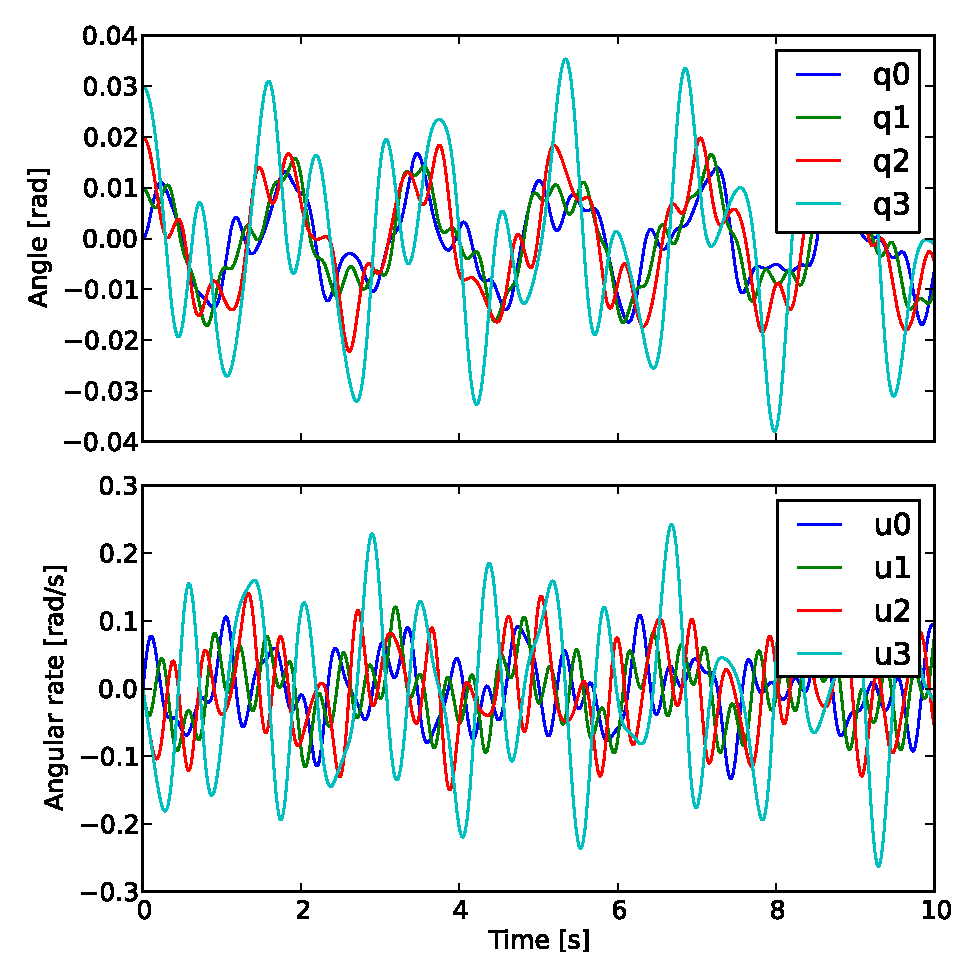
\includegraphics[width=\columnwidth]{four_link_pendulum_time_series}
  \caption{Time history of generalized cooridinates and speeds for 4 link
pendulum.}
  \label{fig:time_series}
\end{figure}

Using other Python packages, such as Mayavi, 3D animations can be created. Use
of human-interface-devices (with a sufficiently fast computer) allows for
real-time interaction between a user and a visualized simulation.

%%%%%%%%%%%%%%%%%%%%%%%%%%%%%%%%%%%%%%%%%%%%%%%%%
\section*{SOFTWARE VALIDATION}
Anytime new software is developed to generate equations of motion, the validity
and accuracy of the software comes into question. We have addressed these
concerns in three ways to ensure that our code does generate correct equations
of motion for arbitrarily complex systems. Firstly, the code is open source and
well documented. This allows anyone to review the code and check for bugs.
Linus's Law ``given enough eyeballs, all bugs are shallow'' \cite{Raymond1999}
applies, if true. Secondly, the code functionality is thoroughly checked with
unit testing; each piece of independent functionality in the code has a test
(known input/output) in place that guarantees correct functioning of each unit.
This ensures that not only the current code works as expected, but also that
future versions are automatically checked against the same expected behavior.
Thirdly, there are built in tests for well benchmarked problems in mutlibody
dynamics. There are many problems, both simple and complex, that have well
known symbolic solutions. We have chosen several benchmark problems that
include sequential rotations, configuration and motion constraints, and
examination of noncontributing forces. These problems are built into the test
suite for the package.

Built in tests which validate the equations of motion that are generated
include: varying degrees of freedom spring-mass-damper systems, various
pendulums, multiple rolling disc examples testing auxiliary and dependent
speeds, and an inverted-pendulum cart. These are all compared to results found
by hand (checked multiple times). The other parts of sympy.physics.mechanics
include hundreds of tests on other pieces of the overall functionality.

There are also some external (non-automated) tests which are more advanced.
Currently, the most complicated test validates the formulation of the equations
of motion for a bicycle (a system with configuration and velocity constraints),
symbolically linearizes it, and compares it (successfully) to benchmark values
\cite{Meijaard2007}.

%%%%%%%%%%%%%%%%%%%%%%%%%%%%%%%%%%%%%%%%%%%%%%%%%%%%%%%%%%%%%%%%%%%%%%%%%%%%%%
\section*{USAGE}
%%%%%%%%%%%% JASON BELOW HERE %%%%%%%%%%%%
This section deals with obtaining the software demonstrated in this paper and
the available resources for learning to use it. All of the software
demonstrated in this paper can be readily obtained for free and installed on
virtually any platform. Also, all of the packages are liberally licensed with a
BSD or compatible license and either stable releases or development branches
can be downloaded.

To obtain and use the core \verb|mechanics| package for symbolic equation of
motion generation, one must simply download and install Python version 2.5+ and
SymPy version 0.7.2+\footnote{One of the major requirements for code added to
SymPy is that every function and object has to be thoroughly tested and
documented. SymPy has over 88\% of its code tested by the automated unit-tests.
This ensures that no update causes regressions or breaks current functionality.
Generally, the SymPy development branch is more stable and contains less bugs
than the numbered releases.}. Download and installation instructions for each
can be found on the softwares' respective web sites, www.python.org and
www.sympy.org.

To run a full PyDy example from equation of motion generation to simulation and
visualization, Python and at least the scientific Python (SciPy) software stack
http://scipy.github.com/stackspec.html must be obtained. We make use of these
packages in the SciPy stack in the previous demo problem:
%
\begin{itemize}
  \item SymPy: http://sympy.org/
  \item NumPy: http://www.numpy.org/
  \item SciPy: http://www.scipy.org/
  \item matplotlib: http://matplotlib.org/
\end{itemize}

Download and installation instructions for various platforms are available on
their respective web sites. But it is worth noting that these packages are a
part of most of the widely used scientific Python distributions. Downloading a
distribution binary is generally the easiest method of installing \emph{all} of
the needed software for a user unfamiliar with Python.
Popular scientific distributions that provide the needed software are listed
below:
%
\begin{itemize}
  \item Enthought: http://www.enthought.com/
  \item Sage: http://www.sagemath.org/
  \item Anaconda: http://continuum.io/
  \item Python(x,y): http://www.pythonxy.com
\end{itemize}

SciPy provides more comprehensive installation instructions than space permits
here: http://scipy.github.com/install.html.

The first step in doing multibody dynamics with Python is to get familiar using
\verb|mechanics|\footnote{Some may prefer to learn Python and the SciPy Stack
first, but the authors do not think this is such a necessity. It boils down to
preference and learning style}. The first stop is the SymPy documentation which
is available online at http://docs.sympy.org/. The documentation provides
detailed instructions on installation, has introductory tutorials, lists common
mistakes, details development procedures and the internal architecture, and
contains detailed documentation for all of the subpackages and modules. In
particular, the \verb|mechanics| documentation contains over 60 pages that aim
to provide an overview of using the package and a brief introduction to the
fundamentals dynamics. Several example classic dynamics problems are included
in the documentation and there are even more in the \verb|mechanics.tests|
package. Working through the material in the \verb|mechanics| documentation
will provide the basics of generating the symbolic equations of motion of
multibody systems.

Additionally, a wiki for PyDy is maintained at www.pydy.org. This is a
user-editable guide to solving dynamics problems in Python, and contains
numerous introductory examples that demonstrate the process from system
definition to simulation and visualization, examples of interfacing
\verb|mechanics| with various compiled languages, and more advanced use cases
to demonstrate capabilities. As the PyDy workflow is integrated into more
university courses, the goal is to allow professors, teaching assistants, and
students to utilize, refine, and expand the wiki.

Finally, each of the software packages listed above maintains email lists and
IRC channels for ``live'' help and the communities supporting the software are
quite amicable to beginners. The PyDy Google Group is a good place to start if
you have questions \cite{PyDyGoogleGroup}.
%
\section*{SOFTWARE DESIGN}
The software design for \verb|mechanics| is influenced by Python's object
oriented nature, the underlying SymPy data types, Kane's method for generating
equations of motion\cite{Kane1985} for multibody systems, and the proprietary
(now defunct) software, Autolev\cite{Kane2000}, which also implemented Kane's
method in a symbolic fashion.

Kane's method powers many of the dynamic system software packages available
\cite{Sayers1990, Enlighten2013} due to its detailed bookkeeping design and
ease of mapping to programming languages. Kane's method  has influenced the
design of \verb|mechanics| a great deal, but the code is structured so that any
method for deriving the equations could be used.  This is possible because we
separated the kinematic code from the equations of motion generation code. We
have recently included Lagrange’s method to demonstrate that unique ability.

SymPy's symbolic manipulation library provides the core functionality for the
mechanics package. The majority of objects that are created when using SymPy
are expression objects, \verb|Expr|. Other symbolic objects in SymPy, such as
symbols, adds and muls, or exponentials are inherited from the \verb|Expr|
class. The \verb|mechanics| package is dependent on these objects, but not via
inheritance. \verb|mechanics| is made up of a number of classes and functions
spread out over several modules which are explained in the following list:
%
\begin{description}
  \item[essential.py] contains the basic building blocks for working with
    vector calculus and dynamic systems and includes the following classes and
    functions:
    \begin{description}
      \item[ReferenceFrame] is a class that represent a rotational reference
        frame in a dynamic system. \verb|ReferenceFrame| has three orthonormal
        basis unit vectors and manages information about the frame's
        orientation, angular velocity, and angular acceleration relative to
        other reference frames through a direction cosine matrix and velocity
        and acceleration vectors. It is closely interlinked to the
        \verb|Vector| class, i.e. \verb|Vector|s have associated
        \verb|ReferenceFrame|s and \verb|ReferenceFrames|s have associated
        \verb|Vector|s.
      \item[Vector] is a class that represents a generic three dimensional
        vector built from components in multiple frames of reference. Vectors
        support all of the common operations as one would expect such as
        addition, subtraction, multiplication, division, dot products, cross
        products, outer products, re-expression into different reference
        frames, and frame dependent differentiation.
      \item[Dyadic] is a class that represents a generic Dyadic. Dyadics are
        used in this software as a basis independent method of defining an
        inertia tensor. Dyadics support all of the common operations, much
        similar to the Vector class.
      \item[dynamicsymbols] is a function that is used to facilitate the generation
        of time dependent quantities and their derivatives. This variables are
        created as SymPy \verb|Function|s of time, where the default time is
        the symbols \verb|t|.
    \end{description}
  \item[point.py] contains the \verb|Point| class. This class manages
    and tracks the location, velocity, and acceleration of a point in space
    relative to another point. It also provides some convenience methods to set
    velocities and accelerations via the one point and two point theories
    \cite{Kane1985}.
  \item[functions.py] contains an assortment of convenience functions. For
    example there is a function for generating inertia dyadics from tensor
    notation, a function that outputs kinematical differential equations for
    various body or spaced fixed coordinates and speeds, functions to generate
    linear and angular momenta or kinetic and potential energies for a general
    system of particles and bodies, among others.
  \item[particle.py] contains the \verb|Particle| class which functions as a
    container class for a point and an associated mass. It also has methods for
    computing momentum and energy.
  \item[rigidbody.py] contains the \verb|RigidBody| is analogous to the
    \verb|Particle| class but for rigid bodies and contains mass, mass center,
    inertia, and a reference frame associated with the rigid body. It also has
    methods for momentum and energy.
  \item[kane.py] contains the \verb|KanesMethod| class which automates the
    generation of a system's non-linear equations of motion using Kane's
    method\cite{Kane1985} and linear equations of motion using the method
    presented in \cite{Peterson2013}. A \verb|KanesMethod| object is initialized
    with an inertial reference frame, set of particles and/or rigid bodies, a
    set of forces and torques acting on the system, the desired kinematical
    differential equations, the desired independent and dependent generalized
    speeds, any configuration constraints, any velocity constraints, and any
    auxiliary speeds needed to compute non-contributing forces.
  \item[lagrange.py] contains the \verb|LagrangesMethod| class which automates
    the generation of a system's non-linear equations of motion via the methods
    of Lagrangian mechanics\cite{Crandall1968}. To derive the equations of
    motion of a constrained system using Lagrange's equations, one requires the
    configuration and velocity constraint equations, if any, before proceeding
    to derive a complete set of dynamical equations that describe said system.
    The \verb|LagrangesMethod| object is initialized with a Lagrangian and the
    desired generalized coordinates and optionally forces acting on the system,
    velocity constraints, and an inertial reference frame. If velocity
    constraints are supplied, Lagrange multipliers are generated to account for
    them and non-conservative forces are appropriately handled if applied they
    affect the system.
\end{description}

%%%%%%%%%%%% JASON ABOVE HERE %%%%%%%%%%%%
%%%%%%%%%%%% GILBERT BELOW HERE %%%%%%%%%%
\subsection*{ESSENTIAL}
As previously shown, the submodule essential.py (which is the core of
sympy.physics.mechanics) is made of \verb|ReferenceFrame|, \verb|Vector|,
\verb|Dyadic|, and \verb|dynamicsymbols| (as well as some output functions).
These classes will be explained in some detail, to allow for a greater
understanding of how our software was written and how it functions.

Firstly, \verb|dynamicsymbols| will be explained - it is merely a shortcut to
producing quantities which are functions of time.
It is included in essential for 2 reasons: specifics relating to Python
importing requirements, and because \verb|dynamicsymbols| defines the symbol
used to represent time (default ``t'').
All of the vector calculus methods assume that functions of time define
rotations between \verb|ReferenceFrame|s; if basic symbols or expressions which
are not functions of time are supplied, they will be treated as constants when
differentiating with respect to time.

The relationship between \verb|ReferenceFrame| and \verb|Vector| is very
complex; we will attempt to describe it here.
Upon initialization, a \verb|ReferenceFrame| has 3 vectors which are created,
representing the orthonormal basis vectors of that reference frame.
A \verb|Vector| is made up of a list of segments per frame; for each unique
\verb|ReferenceFrame| involved in the definition of a vector, one element in
this list exists.
Each element in the list contains the associated \verb|ReferenceFrame| and a
$3\times1$ SymPy matrix representing the measure numbers for each frame.
The basis vectors which are created upon \verb|ReferenceFrame| initialization
therefore have a list of length 1, made up of the \verb|ReferenceFrame| they
are created in and a matrix that defines one of the standard basis vectors
(e.g. $[1, 0, 0]$).

As objects, both these basis vectors and other vectors are instances of the
same \verb|Vector| class.
More complicated \verb|Vector|s just consist of longer lists, and matrices
which are not as basic; more frames can be introduced by adding vectors
together or performing more advanced vector and vector calculus operations.

The final two parts of \verb|Vector|'s design are in the users interaction with
these objects - creating and displaying them.
Direct initialization of a \verb|Vector| object by a user should never take
place; more complicated vectors will be formed out of basis vectors from the
\verb|ReferenceFrame|s and operations between \verb|Vector|s.
When displaying a \verb|Vector| object to the user, the complex implementation
details of each instance are masked.
Instead, the user only sees something along the following lines:
\begin{verbatim}
3*A.x + 5*A.y + sin(theta)*C.z
\end{verbatim}
Each measure number and accompanying basis vector are printed out in a way that
the output can be copied and reentered to form the \verb|Vector| again.
This leaves our \verb|Vector| class as a symbolic object (although, not a
subclass of the main SymPy \verb|Expr| class) which users will interact with on
a symbolic/mathematical level; the complex initialization should never have to
be done by hand, making use of this class is easy for people not intimately
familiar with Python and SymPy.

In order to allow interactions between vectors defined in different reference
frames, information is stored which relates each reference frame to others.
The user defines how one frame is oriented to another, using an arbitrary axis,
standard body or space Euler angles, or Euler parameters.
Once this is defined, each of the involved \verb|ReferenceFrame|s sets its
internal dictionary where a pointer to the other frame and the generated
direction cosine matrix are stored together (transposing happens for one of the
frames).
When the orientation matrix between 2 frames is requested, if it has not
already been defined, the code will search through all possible branches to
find the other frame, and then multiply all of the orientation matrices in
order to generate the direction cosine matrix between the two frames.
After doing so, it will be saved so in the future searching does not have to
happen again.

Angular velocities between frames are set in a similar way.
When the user orients one frame relative to another, the angular velocity is
generated by taking the time derivative of the direction cosine matrix.
This is usually not desirable though, so the user is free to overwrite the
angular velocity vector between frames.
Again, setting this in one frame will set an equal and opposite vector in the
other frame, to ensure consistency.
Also, the same tree searching occurs for angular velocities, except it involves
adding angular velocity vectors instead of multiplying direction coside matrices.

One potential pitfall is the possibility of a user closing a loop of
\verb|ReferenceFrame|s.
In doing so, it is possible for the user to create internally inconsistent
rotations or angular velocities; in other terms, if they don't use the correct
value when closing the loop, the code does not detect this and incorrect
results might be generated.
Users are instructed to avoid doing this, and we feel it is an unlikely
scenario, as it requires extra, unneeded work on the user's part.

The \verb|Point| class functions in a similar manner to \verb|ReferenceFrame|,
in that it has a tree which links the position of this points to other points
and is searchable to find the position betwen two points which have not been
directly assigned.
However, the \verb|Point| class does not extend this functionality to
velocities; it only works for positions.
This is due to the complexities of identifying bound/unbound vectors within
reference frames.
It has been more reliable to ask the user to find these velocities themselves
rather than attempting to do it automatically (and frequently incorrectly).
In order to help with this task, the \verb|Point| class has a number of methods
using the one point and two point theorems \cite{Kane1985} to make this step
easier.

The \verb|Dyadic| object has a similar construction approach as \verb|Vector|;
it is made up of a list of components.
However, for a dyadic, there are 3 parts of each list entry: a measure number,
the first basis vector, and the second basis vector.
The lists which compose a \verb|Dyadic| object look like:
\begin{verbatim}
[(J, A.x, A.x), (I, A.x, B.y)]
\end{verbatim}
which in turn is printed as:
\begin{verbatim}
J*(A.x|A.x) + I*(A.x|B.y)
\end{verbatim}
which again follows the SymPy convention that the displayed version of this
object can be copied and pasted in order to remake the object.
The vector math and calculus associated with \verb|Dyadic| is similar to that
in \verb|Vector|; usually either the first or second basis vector is operated
upon, depending on side it is being dotted or crossed.

For a user, once all kinematics and system parameters have been defined, the
next step is generating the equations of motion.
There are two included methods for generating EoM: Kane's and Lagrange's.
Both of these objects require the system's definition to be passed in using the
container classes \verb|Particle| and \verb|RigidBody|.
These objects (as described above) store the minimum amount of information for
a body that is needed to create the equations of motion.

\subsection*{KanesMethod Class}
Upon initialization, it takes in a number of properties which describe the
system: the inertial reference frame; independent and constrained generalized
coordinates; independent, auxiliary, and constrained (dependent) generalized
speeds; and configuration, velocity, and (optionally) acceleration constraint
equations. At this point, the relationships between the independent and
constrained speeds are found as in Kane's Method \cite{Kane1985}; this is shown
in equation (\ref{eq:Ars_forming}), where $f_v(q, u, t)$ is the list of
constraint equations and $u$ is the list of independent and dependent speeds.
\begin{align}
%\begin{subequations}
\mathbf{0} &= f_v(q, u, t) \\
\mathbf{0} &= \nabla_u f_v(q, u, t) \mathbf{u} \\
           &= \mathbf{B} \mathbf{u} \\
\mathbf{0} &= \mathbf{B}_{ind} \mathbf{u}_{ind} + \mathbf{B}_{dep}
\mathbf{u}_{dep} \\
\mathbf{u}_{dep} &= - \mathbf{B}_{dep}^{-1} \mathbf{B}_{ind} \mathbf{u}_{ind} \\
\mathbf{u}_{dep} &= \mathbf{A} \mathbf{u}_{ind}
%\end{subequations}
\label{eq:Ars_forming}
\end{align}
The configuration constraints are not actually important when forming the
equations of motion, but they do need to be supplied if the system is going to
be linearized \cite{Peterson2013}.

From here, the formulation of the term $\mathbf{F}_r$ follows what Kane
presented, with the advantage that all of the vector addition and
multiplication is carried out symbolically.  If necessary, the unconstrained
generalized active forces can be transformed into the constrained generalized
active forces, where $n$ is the total number of generalized speeds, $p$ is the
number of independent speeds, leaving $m$ as the number of constrained speeds;
this is shown in equation (\ref{eq:uncon_to_con}).

\begin{equation}
\label{eq:uncon_to_con}
\tilde{\mathbf{F}}_{ind} = \mathbf{F}_{ind} + \mathbf{A}^{T}
\mathbf{F}_{dep}
\end{equation}

The formulation of the generalized inertia forces is more complicated.
First, we defined $\mathbf{F}_r^*$ differently, as in equation (x).
\begin{equation}
\mathbf{F}_r^* = \mathbf{M}_m \mathbf{\dot{u}} + \mathbf{M}_n
\end{equation}
$\mathbf{M}_m$ is the mass matrix of the system and $\mathbf{M}_n$ is all the
terms in $\mathbf{F}_r^*$ which are not part of the mass matrix.  The
construction of these terms will be shown for a particle, but the procedure for
rigid bodies is almost the same, albeit for the rotational components.  If we
start by defining the velocity of a particle $P$ in the inertial frame $A$ as:
\begin{equation}
^{A}\underline{v}^{P} = \sum_{i=1}^{n} {} ^{A}\underline{v}_{r}^{P}
\end{equation}
the inertial force $R^*$ for that particle can be written as:
\begin{align}
%\begin{subequations}
\underline{R}^* &= -\frac{^{A} d}{dt}(m ^A\underline{v}^P) \\
&= -m \frac{^{A}d}{dt}^A\underline{v}^P - \dot{m} ^A\underline{v}^P \\
&= -\dot{m} ^A\underline{v}^P - m \frac{^{A}d}{dt}\left(\sum_{i=1}^{n}{} ^A
\underline{v}^P_i u_i \right) \\
&= -\dot{m} ^A\underline{v}^P - m \sum_{i=1}^{n} \left( ^A\underline{v}_i^P
\frac{d}{dt}u_i + u_i \frac{^{A}d}{dt} {}^A\underline{v}^P_i \right) \\
%\end{subequations}
\end{align}
We can then write:
\begin{align}
\mathbf{F^*}_r &= ^A\underline{v}^P_r \underline{R}^{*} \\
\mathbf{F^*}_r &= - \left[
                   ^A\underline{v}^P_r \dot{m} ^A\underline{v}^P +
                   ^A\underline{v}^P_r m \sum_{i=1}^{n} \left(
                   \dot{u}_i ^A\underline{v}^P_i + u_i
                   \frac{^{A}d}{dt} {}^A\underline{v}^P_i
                   \right)
                   \right]
\end{align}
While the above equation looks very complicated, it is not difficult to form
computationally.
Observing this equation, we can see that only the mass and partial velocity
terms multiply $\dot{u}$ terms, or that the mass matrix coefficients are made
up of the product of mass and the dot product between two partial velocities.
In fact, the location of the element in the mass matrix corresponds to the
index of each partial velocity (the order is not important as long as it is
consistent).
If we wanted to define this another way, we could write a vertical vector of
the partial velocities of particle $P$, $[^A\underline{v}^P_r]$, and then the
mass matrix would be:
\begin{equation}
\mathbf{M}_m = -m \left[^A\underline{v}_r^P\right] \left[^A\underline{v}_r^P \right]^T
\end{equation}

In either case, the non mass matrix terms (which make up $M_n$) are the
collection of terms that do not involve $\dot{u}$'s.
As in Kane's method, the rotational and translational inertia forces and
torques are multiplied by the angular and translational partial velocities,
done for each body/particle, and then summed for all bodies and particles.
In order to transform this for systems with nonholonomic constraints, we again
use equation (\ref{eq:uncon_to_con}), substituting $\mathbf{F}^*$ for
$\mathbf{F}$.

The use of auxiliary speeds to bring noncontributing forces into evidence is
another important part of utilizing Kane's method.
Upon initialization of a \verb|KanesMethod| object, the user needs to supply
auxiliary speeds.
After that point though, assuming the auxiliary speeds were used correctly when
forming velocities, the user does not have to worry about these speeds again;
they will not show up in any output equations.
One peculiarity that should be noted is the case when we have velocity
constraints and auxiliary speeds.
In order to form the correct auxiliary equations, the relationship between the
auxiliary speeds and the constrained speeds needs to be found and used in
forming the equations.
The way this is implemented within the class is relatively simple.
A second, internal \verb|KanesMethod| object is created which has the same
constraints and constrained speeds, but the auxiliary speeds are supplied as
both independent and auxiliary speeds, leaving the rest of the math the same.

More plainly, for any instance of \verb|KanesMethod|, auxiliary speeds are
removed from (set to 0) the accelerations and velocities that form
$\underline{R}, \underline{T}, \underline{R}^*$, and $\underline{T}^*$.
The only difference between the user's and the internal instance is which
generalized speeds are used to form the partial velocities: independent or
auxiliary.
The relationship between the auxiliary speeds and constrained speeds is found
the same way as the relationship between the independent speeds and constrained
speeds - the matrix $A$ that is found relates auxiliary and constrained
speeds.
Furthermore, the transformation from unconstrained auxiliary equations to the
constrained auxiliary equations ($\mathbf{F} + \mathbf{F}^*=0$ to
$\tilde{\mathbf{F}} + \tilde{\mathbf{F}}^* = 0$ is performed exactly the same
way, just using the matrix $A$ that relates the auxiliary and constrained
speeds.
The entire process is invisible from the user's perspective.

We will only briefly discuss linearization here, as a more detailed description
of the linearization procedure used within \verb|KanesMethod| can be found
elsewhere \cite{Peterson2013}.  The only complications that arise are when the
user has a constrained system, in which case relationships between dependent
and independent coordinates needs to be considered, as well as the relationship
between dependent speeds and independent speeds, independent coordinates, and
dependent coordinates.  The important message for the user is that
configuration constraints are not considered when forming the equations of
motion, but if they exist and are not supplied, the linear equations that are
generated will be incorrect.

As the constrained generalized speeds are not substituted out of the equations
generated, we will have fewer equations then independent and dependent speeds.
If we have $n$ total generalized speeds and $p$ independent speeds, we are left
with $m=n-p$ constrained speeds.
This means that we will have $p$ equations containing time derivatives of $n$
speeds, or not enough equations to solve for the $\dot{u}$'s.
We instead use the $m$ velocity constraint equations to generate the needed
equations.
When the velocity constraint equations are differentiated with respect to time,
we get $m$ equations (the additional number we needed) containing up to $n$
$\dot{u}$'s, giving the required information to solve for the time derivatives
of the generalized speeds.
%%%%%%%%%%%% GILBERT ABOVE HERE %%%%%%%%%%
%%%%%%%%%%%% ANGADH BELOW HERE %%%%%%%%%%%
\subsection*{LangrangesMethod Class}
In sympy.physics.mechanics, we assume that 3 basic sets of equations are
necessary to completely describe a system and obtain the symbolic equations
using \verb|LagrangesMethod|. They are:

\begin{align}
    \label{eqn:lag_qd}
    0 &= \mathbf{m_{c}}(q, t) \dot{q} + \mathbf{f_{c}}(q, t)\\
    \label{eqn:lag_qdd}
    0 &= \mathbf{m_{dc}}(\dot{q}, q, t) \ddot{q} + \mathbf{f_{dc}}(\dot{q}, q,
        t)\\
    \label{eqn:lag_eom}
    0 &= \mathbf{m_d}(\dot{q}, q, t) \ddot{q} + \Lambda_c(q, t)
        \lambda + \mathbf{f_d}(\dot{q}, q, t)
\end{align}

where $q$ represents a vector of generalized coordinates, $\dot{q}$ and
$\ddot{q}$ are vectors of the first and second time derivatives of the
generalized coordinates, $\mathbf{\lambda}$ is a vector of the Lagrange
multipliers. $\mathbf{m_c}$, $\mathbf{m_dc}$, $\mathbf{m_d}$ and
$\Lambda_c$ are coefficient matrices.
Equation (\ref{eqn:lag_qd}) shows the constraint equations,
(\ref{eqn:lag_qdd}) shows the
first derivative of the constraint equations, and (\ref{eqn:lag_eom}) shows
the dynamical equations using Lagrange's equations. The
\verb|LagrangesMethod| class rearranges the equations of motion into the
following form:
\label{eqn:lag_rearr}
\begin{align}
    \mathbf{M}(q, t) x = \mathbf{f}(q, \dot{q}, t)
\end{align}
where $\mathbf{M}$ is the 'mass matrix', and $x$ is a vector of the states,
namely the $\ddot{q}$'s and $\lambda$'s, if any.

\subsection*{ADDITIONAL FEATURES}
Dynamicists have varied tastes when it comes to naming conventions of
orthonormal basis vectors. For example, while some may define $a_i
\quad (i=x,y,z)$ as the basis vectors for a reference frame $A$, others may
choose to define $a_i \quad (i=1,2,3)$ as the basis vectors for the same frame.
This flexibility of indexing reference frames based on personal preference has
been retained in PyDy.

%%Limitations section. Not really certain how to expan too much on it but
%I guess we can talk about it later today in the lab
%\section*{LIMITATIONS}
%In testing PyDy thus far, we have yet to clearly establish the computational
%limitations. The most complex system studied using PyDy so far is the bicycle,
%the derivation of whose linearized equations of motion take approximately
%two minutes.
%
%PyDy lacks the capability of setting up a system by using graphical objects
%(like rigid slender rods, rigid cylinders, etc.) to configure a mechanical
%system. Currently, the study of any dynamical system can only be performed by
%writing a script to configure a system and further study it.

%%%%%%%%%%%% ANGADH ABOVE HERE %%%%%%%%%%%

\section*{CONCLUSIONS}
In this paper, we have presented a set of tools, PyDy, for forming the
equations of motion of a constrained dynamic system in an automated fashion.
The core of PyDy, the mechanics code within SymPy, is written in a high-level
programming language on top of a fully function computer algebra system.
We have demonstrated the use of our software, as well as how it fits into the
larger scientific Python ecosystem.
We also detailed how our software has been validated, why design decisions were
made, and how its internal architecture functions.

\section*{ACKNOWLEDGEMENTS}
Three Google Summer of Code grants (2009, 2011, 2012) supported most of the
software development. This material is also partially based upon work supported
by the National Science Foundation under Grant No. 0928339. Any opinions,
findings, and conclusions or recommendations expressed in this material are
those of the author(s) and do not necessarily reflect the views of the National
Science Foundation.
\bibliographystyle{asmems4}
\bibliography{asme2e}
\end{document}
